
\FloatBarrier
\subsubsection{Система Sprott A}

\LinkRef{
  spr\_a: MKMM-2016
}

В своих работах J.C.~Sprott рассмотрел целое семейство динамических
систем, реализующих хаотическое поведение, обозначив их латинскими буквами
от ``A'' до ``S''~\cite{sprott_212}. Особое место среди них
занимает система, обозначаемая как ``Sprott A''. Отличительной особенностью
этой системы является отсутствие положений равновесия, что делает
невозможным применение многих известных методов анализа, основанных на
каком-либо разложении в окрестностях точек равновесия. Соответствующая ей
система уравнений имеет вид:

\begin{equation}
  \begin{cases}
    \dot{x} =  y, \\
    \dot{y} = -x + yz, \\
    \dot{z} =  1 - y^2.
  \end{cases}
  \label{atu:eq:spr_a_orig}
\end{equation}


В исходном виде система (\ref{atu:eq:spr_a_orig}) имеет фиксированные значения параметров.
Не изменяя структуры системы, можно ввести 5 параметров, влияющие на её динамку. В
данной работе рассмотрим только один -- $c_{x_y} $. Система принимает следующий вид:

\begin{equation}
  \begin{cases}
    \dot{x} =  c_{x_y} y, \\
    \dot{y} = -x + yz, \\
    \dot{z} =  1 - y^2.
  \end{cases}
  \label{atu:eq:spr_a}
\end{equation}

В таком виде система, при изменении $c_{x_y} $
в достаточно широком диапазоне может демонстрировать как
сложно-периодическое, так и преимущественно, хаотическое
поведение (рис.~\ref{atu:f:spr_a_phase}). При этом, в диапазоне $c_{x_y} \in [0.1 ; 0.7] $
наблюдаются перестройки структуры аттрактора, а при относительно больших
значениях данного параметра аттрактор представляет собой полый тор.


\begin{figure}[htb!]
\centerline{
  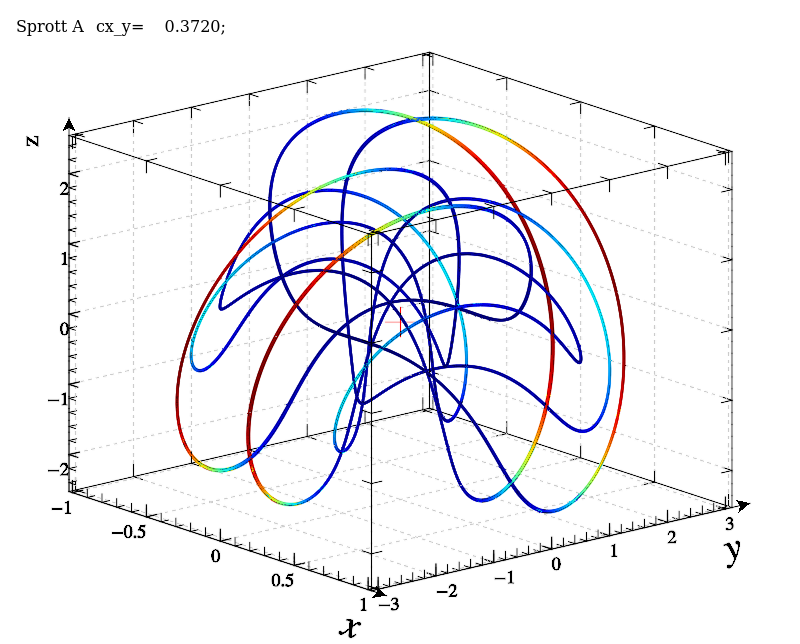
\includegraphics[width=0.33\textwidth]{p/cha/spr_a/sprott_a-p_xyz_cx_y=0x372.png}
  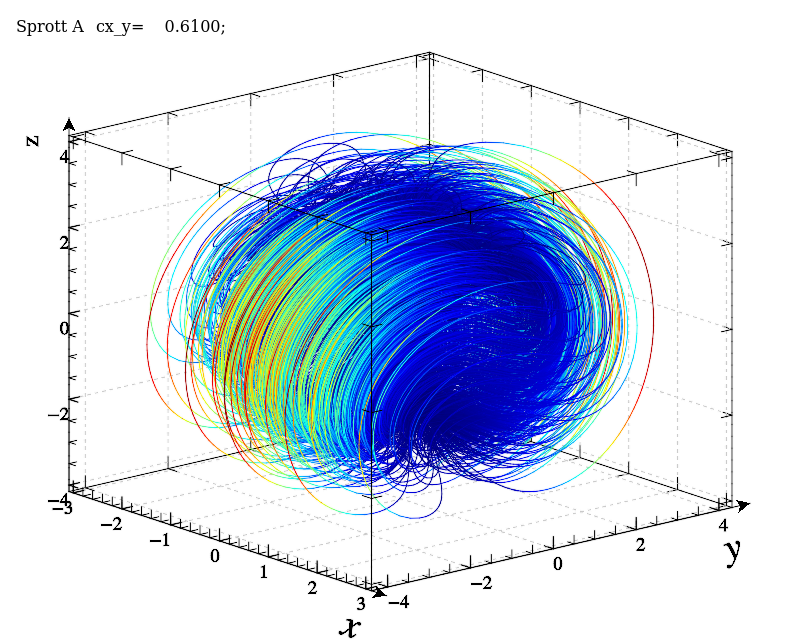
\includegraphics[width=0.33\textwidth]{p/cha/spr_a/sprott_a-p_xyz_cx_y=0x610.png}
  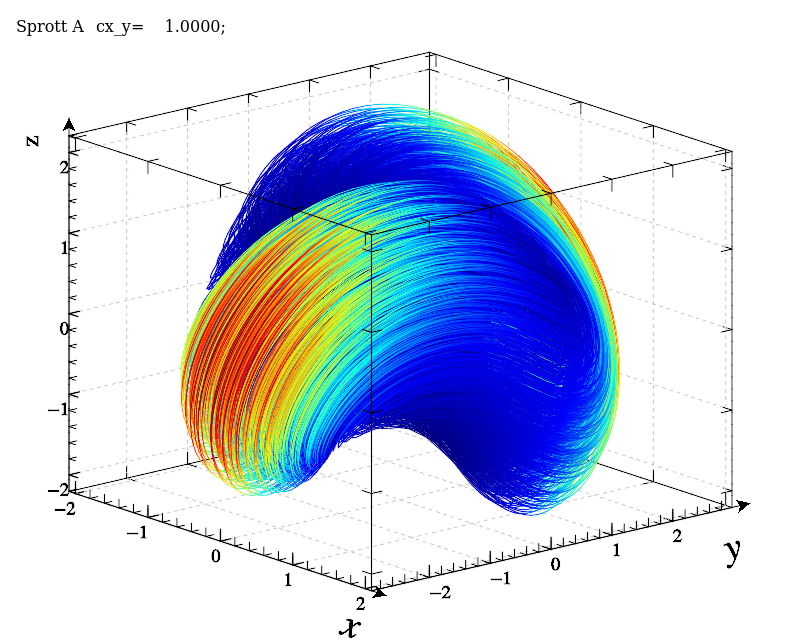
\includegraphics[width=0.33\textwidth]{p/cha/spr_a/sprott_a-p_xyz_cx_y=1x000.png}
}
\caption{Аттракторы системы (\ref{atu:eq:spr_a})
  при $ c_{x_y} =0.372 $, $ c_{x_y} =0.61 $, $ c_{x_y} =1.00 $
}
\label{atu:f:spr_a_phase}
\end{figure}

Важной особенностью поведения этой системы что при $ c_{x_y} \ge 1 $
в спектре системы имеются очень ограниченные участки сплошного спектра~(рис.~\ref{atu:f:spr_a_f}).
При этом, как и для получения корректного спектра, так и для обнаружения разбегания траекторий
необходимо моделирование системы на протяжении достаточно длительного
(по сравнению с многими схожими системами) модельного времени.

\begin{figure}[htb!]
\centerline{
  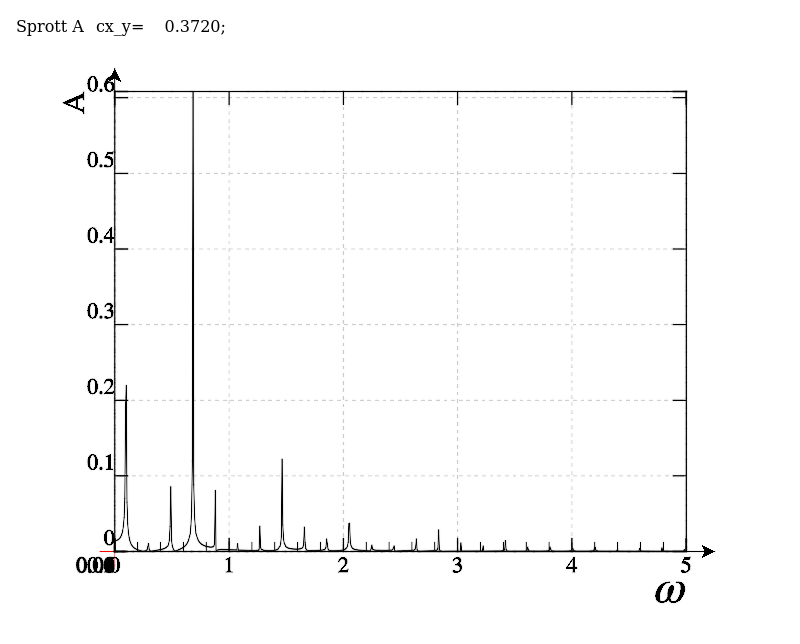
\includegraphics[width=0.33\textwidth]{p/cha/spr_a/sprott_a_f-p_f_cx_y=0x372.png}
  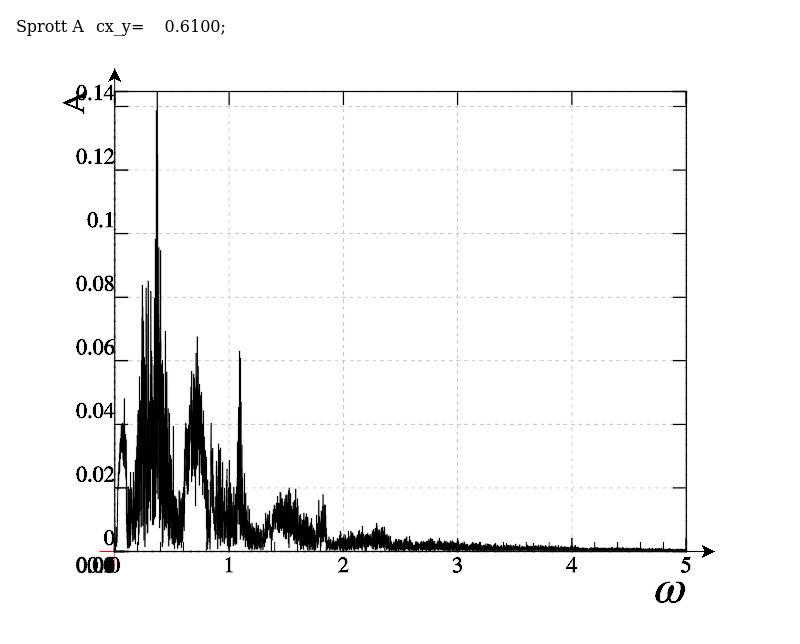
\includegraphics[width=0.33\textwidth]{p/cha/spr_a/sprott_a_f-p_f_cx_y=0x610.png}
  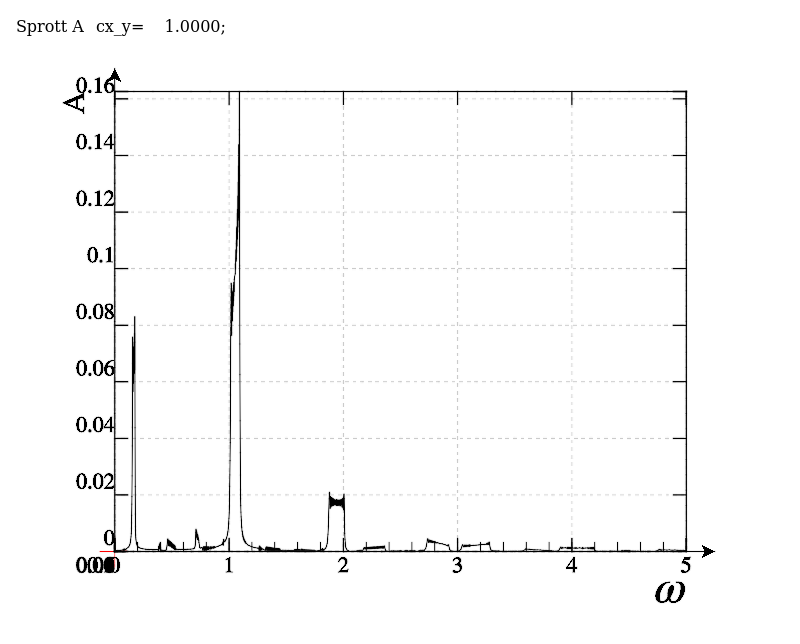
\includegraphics[width=0.33\textwidth]{p/cha/spr_a/sprott_a_f-p_f_cx_y=1x000.png}
}
\caption{Спектры системы (\ref{atu:eq:spr_a})
  при $ c_{x_y} =0.372 $, $ c_{x_y} =0.61 $, $ c_{x_y} =1.00 $
}
\label{atu:f:spr_a_f}
\end{figure}

Рассмотрим зависимости $q_{*}(c_{x_y}) $ (рис.~\ref{atu:f:spr_a_q})
для системы (\ref{atu:eq:spr_a}). Анализ зависимостей
даёт однозначный ответ о возможном виде критерия -- $q_{x^2}$.
Используя его, строим систему идентификации.

\begin{figure}[htb!]
\centerline{
  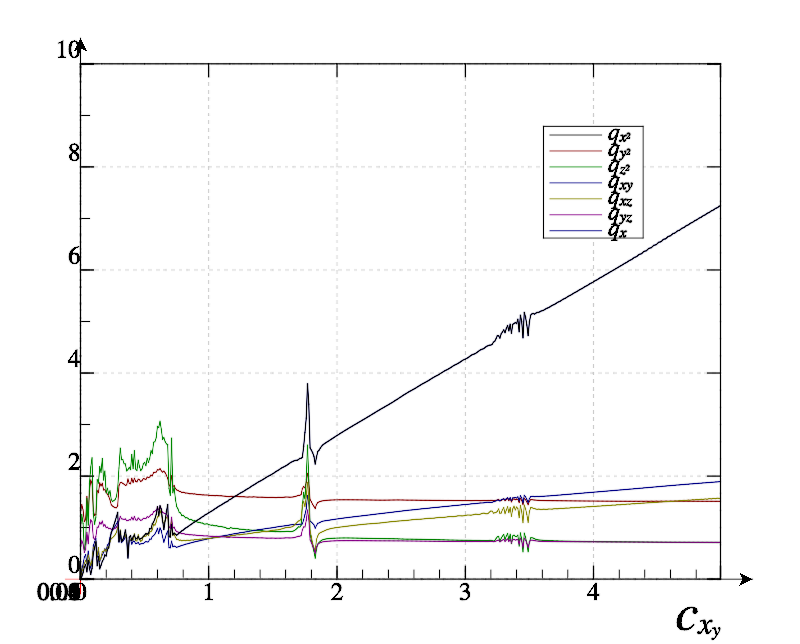
\includegraphics[width=0.50\textwidth]{p/cha/spr_a/sprott_a_p-p_c_x_y.png}
}
\caption{Зависимости $q_{*}(c_{x_y})$ для системы (\ref{atu:eq:spr_a}) }
\label{atu:f:spr_a_q}
\end{figure}


Динамика процессов идентификации для системы Sprott A представлена на рис.~\ref{atu:f:spr_a_id}.
Общий вид динамики поиска свидетельствует о работоспособности системы.

\begin{figure}[htb!]
\centerline{
  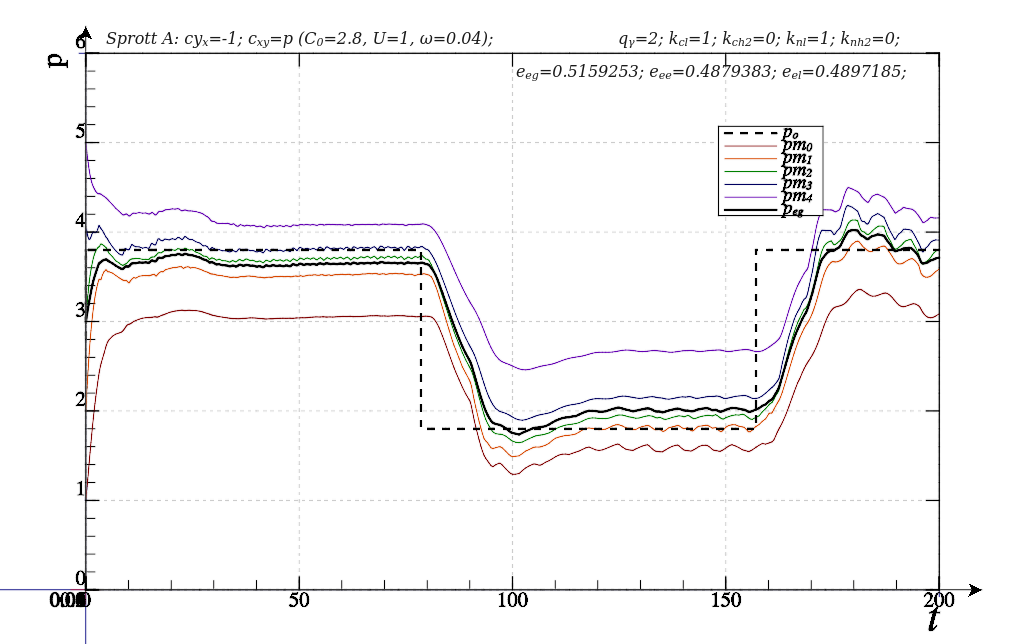
\includegraphics[width=0.49\textwidth]{p/cha/spr_a/sprott_a_m5p-pl_n_sign.png}
  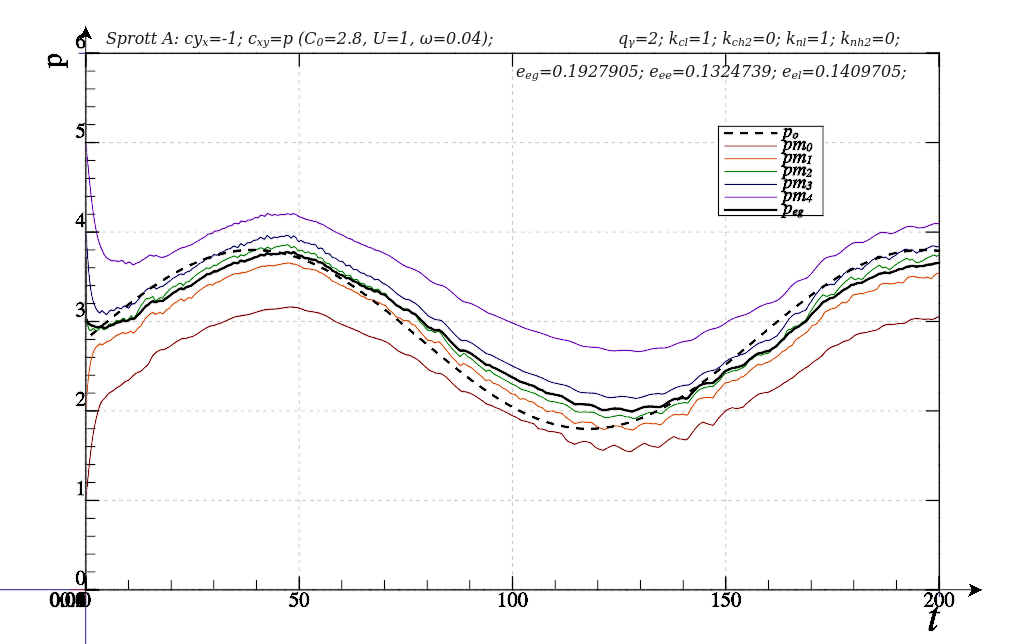
\includegraphics[width=0.49\textwidth]{p/cha/spr_a/sprott_a_m5p-pl_n_sin.png}
}
\caption{Процесс идентификации параметра $c_{x_y} $ системы (\ref{atu:eq:spr_a})
  при различных видах нестационарности этого параметра
}
\label{atu:f:spr_a_id}
\end{figure}

Зависимость среднеквадратических ошибок идентификации от величины $q_\gamma$ (рис.~\ref{atu:f:spr_a_e_qgamma})
свидетельствует о довольно слабой зависимости (в разумных пределах)
динамики системы идентификации о  этого параметра. Скорее всего,
здесь проявляются робастные свойства поисковых агентов.

\begin{figure}[htb!]
\centerline{
  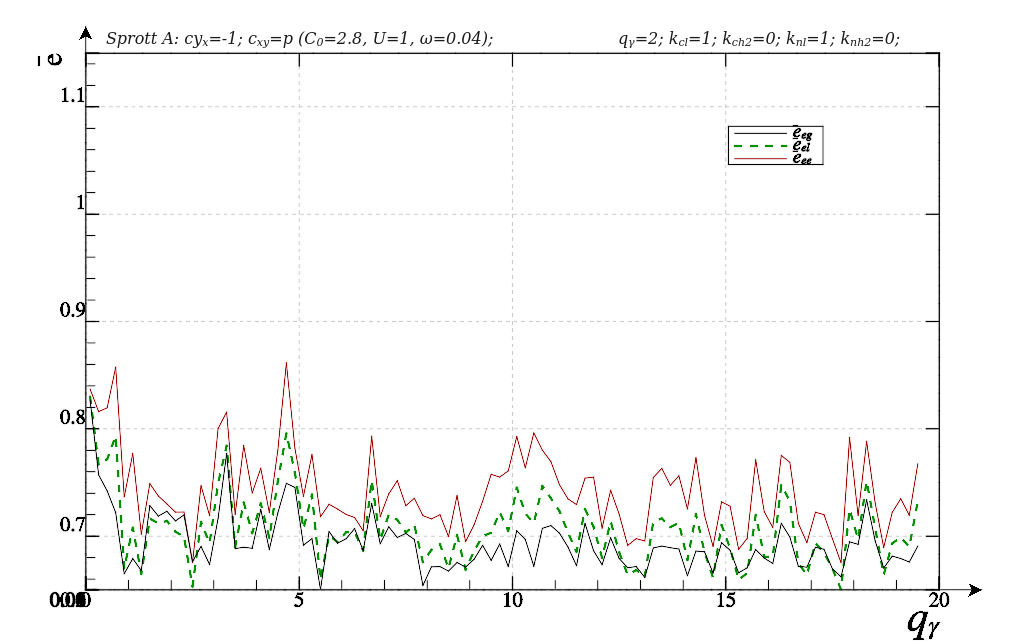
\includegraphics[width=0.49\textwidth]{p/cha/spr_a/sprott_a_m5p-p_qg_e_sign.png}
  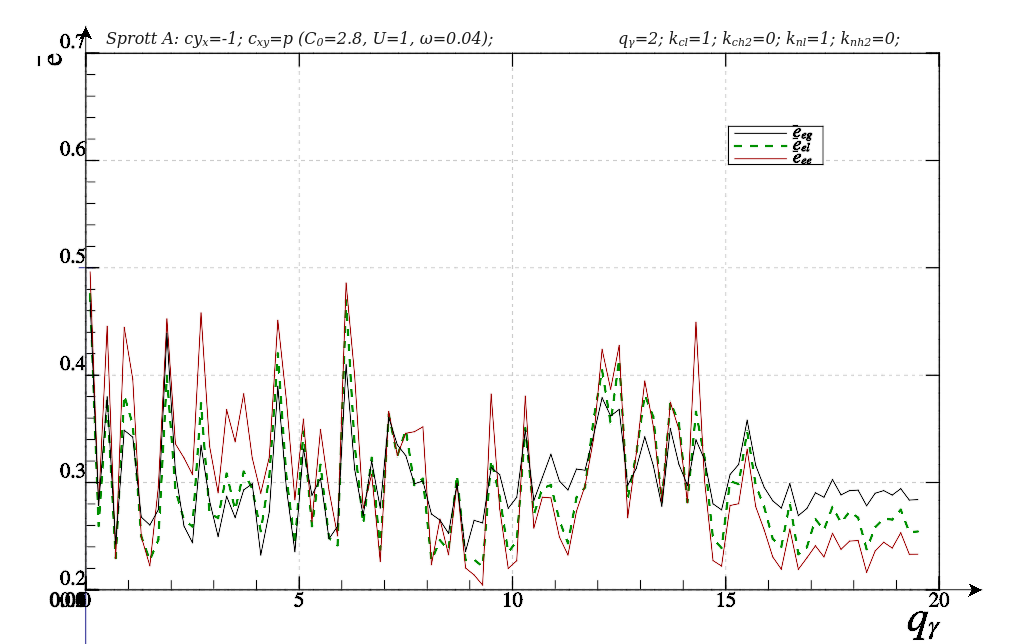
\includegraphics[width=0.49\textwidth]{p/cha/spr_a/sprott_a_m5p-p_qg_e_sin.png}
}
  \caption{Зависимости  $\bar{e}(q_\gamma)$ для системы (\ref{atu:eq:spr_a})
  при различных видах нестационарности этого параметра
}
\label{atu:f:spr_a_e_qgamma}
\end{figure}


Зависимости $\bar{e_*}(a_q)$ (рис.~\ref{atu:f:spr_a_e_a_q})
с одной стороны, позволяют корректно определить время усреденения,
с другой -- подтверждают тезис о том, что более ярко выраженной изменение
параметра требует большего времени наблюдения за системой
для проведения идентификации.

\begin{figure}[htb!]
\centerline{
  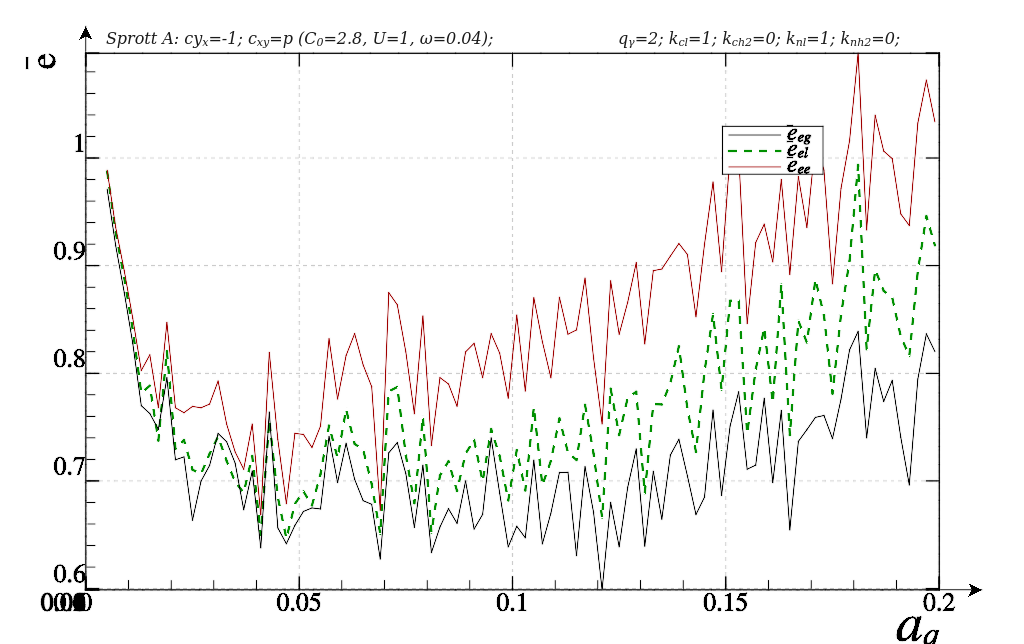
\includegraphics[width=0.49\textwidth]{p/cha/spr_a/sprott_a_m5p-p_a_q_e_sign.png}
  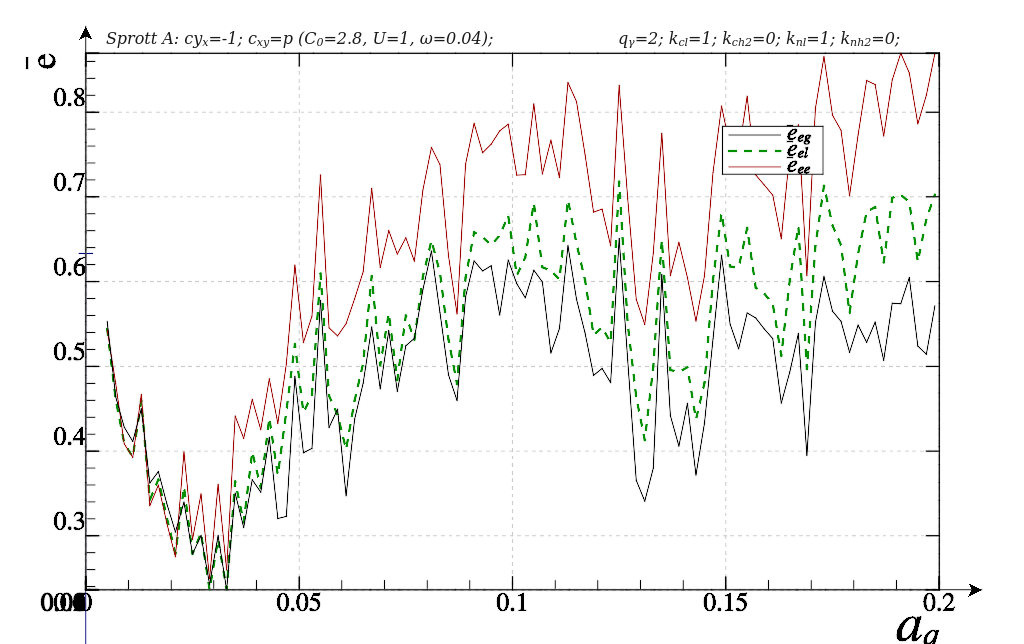
\includegraphics[width=0.49\textwidth]{p/cha/spr_a/sprott_a_m5p-p_a_q_e_sin.png}
}
  \caption{Зависимости  $\bar{e}(a_q)$ для системы (\ref{atu:eq:spr_a})
  при различных видах нестационарности этого параметра
}
\label{atu:f:spr_a_e_a_q}
\end{figure}

И в этом случае удалось создать и критерий идентификации, и работоспособную систему идентификации
на основании энергетического критерия.


